% C17 -- 15 de octubre de 2026. Fragmento del documento principal.
% Fuentes: Screenshots C17/P01--P20.png; Transcripciones/C17.txt.
% La cronología reconstruida y sus incertidumbres constan en C17.txt.
% P02: beta_{n+1} representa un elemento de pi_k(X), no de pi_{k+1}(X).
% P06: se explicita la inversión de caminos respecto de la clase 16.

Probaremos la exactitud de las sucesiones cofibradas en homotopía estable y compararemos la fibra homotópica con la desuspensión de la cofibra. Estas herramientas permitirán demostrar que los productos finitos y los coproductos finitos de espectros son establemente equivalentes, y que los retractos son sumandos. Finalmente construiremos la suma de morfismos estables y comprobaremos que la categoría homotópica estable es aditiva.

Trabajamos con espectros secuenciales y conservamos los modelos de fibras y cofibras de la clase~16. Cuando se requieran modelos bien punteados para las construcciones con conos y smash, se toman los reemplazos correspondientes. Escribiremos $[X,Y]_s$ para los morfismos en $\Ho(\Sp^{\mathbb N})$.

%%%%%%%%%%%%%%%%%%%%%%%%%%%%%%%%%%%%%%%%%%%%%%%%%%%%%%%%%%%%%%%%%%%%%%%%%%%%%%%
\section{Exactitud y comparación de fibras y cofibras}
%%%%%%%%%%%%%%%%%%%%%%%%%%%%%%%%%%%%%%%%%%%%%%%%%%%%%%%%%%%%%%%%%%%%%%%%%%%%%%%

%%%%%%%%%%%%%%%%%%%%%%%%%%%%%%%%%%%%%%%%%%%%%%%%%%%%%%%%%%%%%%%%%%%%%%%%%%%%%%%
\subsection{La sucesión exacta de una cofibra}
%%%%%%%%%%%%%%%%%%%%%%%%%%%%%%%%%%%%%%%%%%%%%%%%%%%%%%%%%%%%%%%%%%%%%%%%%%%%%%%

% P01--P05.
Sea $f\colon X\to Y$ un morfismo de espectros. Recordemos que su cofibra homotópica tiene niveles
\[
(C_f)_n=C_{f_n}=Y_n\cup_{f_n}CX_n,
\qquad
X\xrightarrow{f}Y\xrightarrow{i}C_f.
\]
En este apartado parametrizamos el cono con la base en $t=0$ y el vértice en $t=1$. El cono pegado a $Y_n$ proporciona la nulhomotopía de $i_nf_n$:
\[
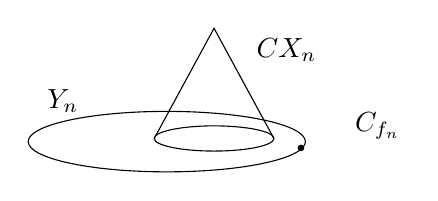
\begin{tikzpicture}[scale=.8,baseline=(current bounding box.center)]
\draw (-2,0) ellipse (2.2 and .48);
\draw (-2.2,.05)--(-1.25,1.8)--(-.3,.05);
\draw (-1.25,.05) ellipse (.95 and .2);
\fill (.13,-.1) circle (1.5pt);
\node at (-3.65,.65) {$Y_n$};
\node at (-.1,1.45) {$CX_n$};
\node at (1.35,.25) {$C_{f_n}$};
\end{tikzpicture}
\]

\begin{prop}\label{prop:c17-exactitud-cofibra}
Toda sucesión cofibrada de espectros induce una sucesión exacta larga natural
\[
\cdots\longrightarrow\pi_k(X)\xrightarrow{f_*}\pi_k(Y)
\xrightarrow{i_*}\pi_k(C_f)\xrightarrow{\partial}\pi_{k-1}(X)
\longrightarrow\cdots.
\]
\end{prop}

\begin{proof}
Basta probar la exactitud en el término central de
\[
\pi_k(X)\xrightarrow{f_*}\pi_k(Y)\xrightarrow{i_*}\pi_k(C_f).
\]
La composición es cero porque $i_nf_n$ es nulhomotópica en cada nivel. Recíprocamente, sea $\alpha\in\pi_k(Y)$ tal que $i_*(\alpha)=0$. Como un elemento nulo en un colímite filtrado se anula en alguna etapa, podemos elegir un representante $\alpha_n$ con $m=k+n\ge2$ y una extensión $\overline\alpha_n$ en el diagrama
\[
\begin{tikzcd}[column sep=large,row sep=large]
S^m\arrow[r,"\alpha_n"]\arrow[d,hook]&Y_n\arrow[r,"i_n"]&C_{f_n}\\
CS^m\arrow[urr,"\overline\alpha_n"']&&
\end{tikzcd}
\]
Introduzcamos las abreviaturas $D_m=CS^m\cup_{S^m}CS^m$ y $E_n=CY_n\cup_{Y_n}C_{f_n}$. La extensión permite pegar los mapas sobre ambos conos y definir
\[
\begin{tikzcd}[column sep=large,row sep=large]
S^{m+1}\arrow[r,"\cong"]\arrow[rrdd,"\beta_{n+1}"']
&D_m\arrow[r,"C\alpha_n\cup\overline\alpha_n"]&E_n\arrow[d,"c_X","\simeq"']\\
&&\Sigma X_n\arrow[d,"\xi_n^X"]\\
&&X_{n+1}.
\end{tikzcd}
\]
Aquí $c_X$ colapsa el primer cono, $CY_n$, y después identifica el cociente con $\Sigma X_n$. El mapa $\beta_{n+1}$ representa una clase en $\pi_{k+n+1}(X_{n+1})$, cuya imagen estable es $\beta\in\pi_k(X)$. Veremos que $f_*(\beta)=\pm\alpha$; el signo no afecta la pertenencia a la imagen.

Definamos $\varphi\colon C_{f_n}\to CY_n$ por $\varphi(y)=[y,0]$ sobre $Y_n$ y $\varphi([x,t])=[f_n(x),t]$ sobre el cono. Las fórmulas coinciden en la base y dan el diagrama
\[
\begin{tikzcd}[column sep=large,row sep=large]
S^{m+1}\arrow[d,"\cong"']&&&\\
D_m\arrow[r,"C\alpha_n\cup\overline\alpha_n"]
&E_n\arrow[r,"c_X","\simeq"']\arrow[d,"\id\cup\varphi"']
&\Sigma X_n\arrow[r,"\xi_n^X"]\arrow[d,"\Sigma f_n"]
&X_{n+1}\arrow[d,"f_{n+1}"]\\
&CY_n\cup_{Y_n}CY_n\arrow[r,"c_N","\simeq"']
&\Sigma Y_n\arrow[r,"\xi_n^Y"']&Y_{n+1}.
\end{tikzcd}
\]
Las identificaciones con las suspensiones se eligen compatibles para que los cuadrados conmuten. Invertir una coordenada de suspensión cambia el signo del representante, lo cual explica la ambigüedad anterior.

Podemos sustituir el colapso del primer cono por el del segundo. Para verlo, identifiquemos el doble cono reducido con una suspensión:
\[
CY_n\cup_{Y_n}CY_n
\cong (CS^0\wedge Y_n)\cup_{S^0\wedge Y_n}(CS^0\wedge Y_n)
\cong S^1\wedge Y_n.
\]
Colapsar uno de los dos semicírculos de $S^1$, orientando el círculo cociente de manera compatible, da un mapa de grado uno. Los dos colapsos son homotópicos; al hacer smash con $Y_n$ obtenemos los triángulos homotópicamente conmutativos
\[
\begin{tikzcd}[column sep=large,row sep=large]
S^1\arrow[r,"c_N"]\arrow[d,equal]&S^1\\
S^1\arrow[ur,"c_S"']&
\end{tikzcd}
\qquad
\begin{tikzcd}[column sep=huge,row sep=large]
S^1\wedge Y_n\arrow[r,"c_N\wedge\id"]\arrow[d,equal]&S^1\wedge Y_n\\
S^1\wedge Y_n\arrow[ur,"c_S\wedge\id"']&
\end{tikzcd}
\]
Salvo homotopía y la elección de orientación, la ruta inferior queda así:
\[
\begin{tikzcd}[column sep=large,row sep=large]
D_m\arrow[r,"C\alpha_n\cup\overline\alpha_n"]&E_n\arrow[d,"\id\cup\varphi"]&&\\
&CY_n\cup_{Y_n}CY_n\arrow[r,"c_S"']&\Sigma Y_n\arrow[r,"\xi_n^Y"']&Y_{n+1}.
\end{tikzcd}
\]
Ahora se colapsa el cono que contiene $\varphi\overline\alpha_n$ y solo queda la suspensión de $\alpha_n$. La composición representa $\pm[\xi_n^Y\Sigma\alpha_n]=\pm[\alpha_{n+1}]$. Al pasar al colímite resulta $f_*(\beta)=\pm\alpha$, y por tanto $\ker i_*\subseteq\im f_*$.

Finalmente, iteramos las cofibras en la sucesión de Puppe. Los isomorfismos $\pi_k(\Sigma X)\cong\pi_{k-1}(X)$ y la exactitud recién probada en cada terna producen la sucesión larga. La naturalidad de los conos, los cocientes y los mapas estructurales asegura la de los homomorfismos de conexión.
\end{proof}

La afirmación análoga para sucesiones fibradas ya se resolvió en el \myref{ejer:c16-sucesiones-fibradas}: se toman las sucesiones exactas nivel a nivel, se pasa al colímite filtrado y se identifican los términos de lazos. Aplicaremos esa solución a la fibra de $f$ en la siguiente comparación.

%%%%%%%%%%%%%%%%%%%%%%%%%%%%%%%%%%%%%%%%%%%%%%%%%%%%%%%%%%%%%%%%%%%%%%%%%%%%%%%
\subsection{La suspensión de la fibra y la cofibra}
%%%%%%%%%%%%%%%%%%%%%%%%%%%%%%%%%%%%%%%%%%%%%%%%%%%%%%%%%%%%%%%%%%%%%%%%%%%%%%%

% P06--P07.
\begin{prop}\label{prop:c17-fibra-cofibra}
Todo morfismo $f\colon X\to Y$ admite una comparación natural $\varepsilon\colon\Sigma F_f\to C_f$ que es una equivalencia estable. En consecuencia, las sucesiones cofibradas y las sucesiones fibradas coinciden en la categoría homotópica estable.
\end{prop}

\begin{proof}
Para escribir la fórmula de la pizarra, usamos el camino inverso al de la clase~16: si allí $\lambda$ va de $f_n(x)$ a $*$, ahora ponemos $\gamma(t)=\lambda(1-t)$. Asimismo, en esta fórmula parametrizamos el cono con base en $u=1$ y vértice en $u=0$. Son cambios de parametrización de los mismos modelos. En estas coordenadas, la fibra queda descrita por
\[
(F_f)_n=\{(x,\gamma):\gamma(0)=*,\ \gamma(1)=f_n(x)\},
\]
y definimos $\varepsilon_n\colon\Sigma(F_f)_n\to Y_n\cup_{f_n}CX_n$ mediante
\[
\varepsilon_n([t,x,\gamma])=
\begin{cases}
\gamma(2t),&0\le t\le\frac12,\\
[x,2-2t],&\frac12\le t\le1.
\end{cases}
\]
En el punto de empalme ambas expresiones representan $f_n(x)$; los extremos y el punto base se envían al punto base. El lema de pegado da continuidad, y la fórmula desciende a la suspensión reducida. El camino recorre primero $\gamma$ en $Y_n$ y luego sube al vértice del cono $CX_n$.

Comprobemos también la compatibilidad con la estructura de espectro, indicada en clase. El mapa estructural de la fibra envía $[s,(x,\gamma)]$ al par formado por $\xi_n^X([s,x])$ y el camino $v\mapsto\xi_n^Y([s,\gamma(v)])$. En la primera mitad de la fórmula de $\varepsilon$ aparece, por cualquiera de las dos composiciones, $\xi_n^Y([s,\gamma(2t)])$; en la segunda aparece el punto del cono $[\xi_n^X([s,x]),2-2t]$. Con la permutación usual de las coordenadas de suspensión, las dos expresiones coinciden. Así, los $\varepsilon_n$ definen un morfismo de espectros, natural en los cuadrados de morfismos $f$.

La sucesión fibrada y su suspensión se comparan con la sucesión cofibrada:
\[
\Omega X\xrightarrow{\Omega f}\Omega Y\longrightarrow F_f
\longrightarrow X\xrightarrow{f}Y,
\]
\[
\begin{tikzcd}[column sep=large,row sep=large]
\Sigma\Omega X\arrow[r,"\Sigma\Omega f"]\arrow[d,"e_X"',"\simeq"]
&\Sigma\Omega Y\arrow[r]\arrow[d,"e_Y"',"\simeq"]
&\Sigma F_f\arrow[r]\arrow[d,"\varepsilon"]
&\Sigma X\arrow[r,"\Sigma f"]\arrow[d,"\rho_X"]
&\Sigma Y\arrow[d,"\rho_Y"]\\
X\arrow[r,"f"']&Y\arrow[r,"i"']&C_f\arrow[r]&\Sigma X\arrow[r,"\Sigma f"']&\Sigma Y.
\end{tikzcd}
\]
El diagrama conmuta salvo homotopía, con las convenciones compatibles de la sucesión de Puppe. Aquí $e_Z\colon\Sigma\Omega Z\to Z$ es la counidad y $\rho_Z([t,z])=[1-t,z]$ es la reflexión de la suspensión, que induce el signo $-1$. El cuadrado que contiene el cociente $C_f\to\Sigma X$ requiere esa reflexión: al colapsar $Y$, la segunda mitad de $\varepsilon$ recorre el cono en sentido inverso.

Las counidades son equivalencias estables. En efecto, los isomorfismos de suspensión y lazos identifican el homomorfismo que inducen con
\[
\pi_k(\Sigma\Omega Z)\cong\pi_{k-1}(\Omega Z)\cong\pi_k(Z),
\]
con las convenciones de signo correspondientes. Las reflexiones son isomorfismos. Ambas filas del diagrama inducen sucesiones exactas en homotopía estable; el lema de los cinco demuestra que $\varepsilon$ también es una equivalencia estable.

La comparación es compatible, salvo las reflexiones señaladas, con los mapas de las sucesiones. Puesto que suspensión y lazos son inversos en la categoría homotópica estable, podemos identificar la fibra con la desuspensión de la cofibra y pasar entre las sucesiones de Puppe fibrada y cofibrada. Esto da la coincidencia afirmada, entendida en dicha categoría.
\end{proof}

%%%%%%%%%%%%%%%%%%%%%%%%%%%%%%%%%%%%%%%%%%%%%%%%%%%%%%%%%%%%%%%%%%%%%%%%%%%%%%%
\section{Productos, coproductos y sumandos estables}
%%%%%%%%%%%%%%%%%%%%%%%%%%%%%%%%%%%%%%%%%%%%%%%%%%%%%%%%%%%%%%%%%%%%%%%%%%%%%%%

%%%%%%%%%%%%%%%%%%%%%%%%%%%%%%%%%%%%%%%%%%%%%%%%%%%%%%%%%%%%%%%%%%%%%%%%%%%%%%%
\subsection{La equivalencia entre el coproducto y el producto finitos}
%%%%%%%%%%%%%%%%%%%%%%%%%%%%%%%%%%%%%%%%%%%%%%%%%%%%%%%%%%%%%%%%%%%%%%%%%%%%%%%

% P08--P10.
Para espectros $X$ y $Y$, el coproducto tiene niveles $(X\vee Y)_n=X_n\vee Y_n$. Su estructura procede de que la suspensión preserva coproductos:
\[
\begin{tikzcd}[column sep=huge,row sep=large]
\Sigma(X_n\vee Y_n)\arrow[r]\arrow[d,"\cong"']&X_{n+1}\vee Y_{n+1}\\
\Sigma X_n\vee\Sigma Y_n\arrow[ur,"\xi_n^X\vee\xi_n^Y"']&
\end{tikzcd}
\]
El producto tiene niveles $(X\times Y)_n=X_n\times Y_n$. Es más cómodo describir su estructura mediante los adjuntos de los mapas estructurales:
\[
\begin{tikzcd}[column sep=large,row sep=large]
X_n\times Y_n\arrow[r,"(\xi_n^X)^\dashv\times(\xi_n^Y)^\dashv"]\arrow[dr]
&\Omega X_{n+1}\times\Omega Y_{n+1}\arrow[d,"\theta","\cong"']\\
&\Omega(X_{n+1}\times Y_{n+1}).
\end{tikzcd}
\]
El isomorfismo $\theta$ asocia a dos lazos el lazo dado por sus dos coordenadas. Las inclusiones $a_n\colon X_n\vee Y_n\to X_n\times Y_n$ son compatibles con estas estructuras:
\[
\begin{tikzcd}[column sep=huge,row sep=large]
\Sigma(X_n\vee Y_n)\arrow[r,"\Sigma a_n"]\arrow[d,"\xi_n^{X\vee Y}"']
&\Sigma(X_n\times Y_n)\arrow[d,"\xi_n^{X\times Y}"]\\
X_{n+1}\vee Y_{n+1}\arrow[r,"a_{n+1}"']&X_{n+1}\times Y_{n+1}.
\end{tikzcd}
\]
Sobre el primer sumando, ambas rutas envían $[s,x]$ a $(\xi_n^X([s,x]),*)$; sobre el segundo, envían $[s,y]$ a $(*,\xi_n^Y([s,y]))$. Tenemos así un morfismo de espectros $a\colon X\vee Y\to X\times Y$.

\begin{prop}\label{prop:c17-coproducto-producto}
La inclusión canónica $a\colon X\vee Y\to X\times Y$ es una equivalencia estable. Además, las inclusiones y las proyecciones inducen isomorfismos
\[
\pi_k(X)\oplus\pi_k(Y)\cong\pi_k(X\vee Y),
\qquad
\pi_k(X\times Y)\cong\pi_k(X)\times\pi_k(Y).
\]
\end{prop}

\begin{proof}
Consideremos los homomorfismos inducidos por las inclusiones y las proyecciones:
\[
\varphi(u,v)=(\iota_1)_*u+(\iota_2)_*v,
\qquad F=((p_1)_*,(p_2)_*).
\]
Junto con $\psi=a_*$, forman el diagrama de la pizarra:
\[
\begin{tikzcd}[column sep=huge,row sep=large]
\pi_k(X)\oplus\pi_k(Y)\arrow[r,"\varphi"]\arrow[rdd,"\cong"']
&\pi_k(X\vee Y)\arrow[d,"\psi=a_*"]\\
&\pi_k(X\times Y)\arrow[d,"F"]\\
&\pi_k(X)\times\pi_k(Y).
\end{tikzcd}
\]
La composición es el isomorfismo canónico: cada inclusión seguida de su proyección da la identidad, y las composiciones cruzadas son cero. Basta demostrar que $\varphi$ y $F$ son isomorfismos.

Para el primero tomamos la sucesión cofibrada
\[
X\xrightarrow{\iota_1}X\vee Y\longrightarrow C_{\iota_1}.
\]
En cada nivel se tiene
\[
(C_{\iota_1})_n=(X_n\vee Y_n)\cup_{\iota_1}CX_n
\cong CX_n\vee Y_n\xrightarrow{\ \simeq\ }Y_n.
\]
El último mapa colapsa el cono y define una equivalencia nivel a nivel $C_{\iota_1}\to Y$. Mediante esta equivalencia obtenemos la sucesión cofibrada
\[
\begin{tikzcd}[column sep=huge]
X\arrow[r,"\iota_1"]&X\vee Y\arrow[r,"c",shift left=.6ex]
&Y\arrow[l,"\iota_2",shift left=.6ex],
\end{tikzcd}
\qquad c\iota_2=\id_Y,
\]
donde $c$ colapsa $X$. La sección hace que todos los homomorfismos de conexión sean cero, de modo que la sucesión larga se descompone en sucesiones exactas cortas escindidas:
\[
\begin{tikzcd}[column sep=small]
0\arrow[r]&\pi_k(X)\arrow[r,"(\iota_1)_*"]&\pi_k(X\vee Y)
\arrow[r,"c_*",shift left=.6ex]&\pi_k(Y)\arrow[l,"(\iota_2)_*",shift left=.6ex]\arrow[r]&0.
\end{tikzcd}
\]
El isomorfismo asociado a esta escisión es precisamente $\varphi$.

Para las proyecciones usamos la comparación
\[
\begin{tikzcd}[column sep=large,row sep=large]
\pi_k(X\times Y)\arrow[r,equal]\arrow[dd,"F"']
&\varinjlim\nolimits_n\pi_{k+n}(X_n\times Y_n)\arrow[d,"\cong"]\\
&\varinjlim\nolimits_n\bigl(\pi_{k+n}(X_n)\times\pi_{k+n}(Y_n)\bigr)\arrow[d,"\cong"]\\
\pi_k(X)\times\pi_k(Y)\arrow[r,equal]
&\bigl(\varinjlim\nolimits_n\pi_{k+n}(X_n)\bigr)\times
\bigl(\varinjlim\nolimits_n\pi_{k+n}(Y_n)\bigr).
\end{tikzcd}
\]
La última identificación usa que los colímites filtrados conmutan con productos finitos. Concretamente, dos representantes pueden llevarse a una misma etapa tomando un índice mayor que ambos; si sus imágenes son cero, también se anulan simultáneamente en una etapa posterior. Esto prueba sobreyectividad e inyectividad. Así, $F$ es un isomorfismo y lo mismo vale para $\psi$.
\end{proof}

\begin{obs}
El resultado se refiere al producto de espectros. Para espacios punteados bien basados, la descomposición recordada en clase es
\[
\Sigma(U\times V)\simeq\Sigma U\vee\Sigma V\vee\Sigma(U\wedge V).
\]
Después de pasar a espectros de suspensión y desuspender queda el sumando $\Sigma^\infty(U\wedge V)$. Los otros dos sumandos se identifican con $\Sigma^\infty U\times\Sigma^\infty V$ por la proposición. Por eso no se debe identificar en general $\Sigma^\infty(U\times V)$ con ese producto: la suspensión infinita no elimina el tercer sumando.
\end{obs}

%%%%%%%%%%%%%%%%%%%%%%%%%%%%%%%%%%%%%%%%%%%%%%%%%%%%%%%%%%%%%%%%%%%%%%%%%%%%%%%
\subsection{Los retractos son sumandos en homotopía estable}
%%%%%%%%%%%%%%%%%%%%%%%%%%%%%%%%%%%%%%%%%%%%%%%%%%%%%%%%%%%%%%%%%%%%%%%%%%%%%%%

% P11--P14; el argumento del toro se pidió como ejercicio.
\begin{ejer}\label{ejer:c17-toro}
La inclusión $i\colon S^1\to S^1\times S^1$, dada por $i(z)=(z,1)$, admite la retracción $r(z,w)=z$. Demostrar que, a pesar de ello, no existe un espacio punteado $Z$ tal que $S^1\times S^1\simeq S^1\vee Z$.
\end{ejer}

\begin{sol}
La composición de los mapas del diagrama es la identidad:
\[
\begin{tikzcd}[column sep=huge]
S^1\arrow[r,"i"]&S^1\times S^1\arrow[r,"r"]&S^1.
\end{tikzcd}
\]
Usamos cohomología racional para descartar la descomposición. El anillo del toro es
\[
H^*(S^1\times S^1;\mathbb Q)\cong\Lambda_{\mathbb Q}(a,b),
\qquad |a|=|b|=1,\quad ab\ne0.
\]
Una equivalencia con $S^1\vee Z$ daría un isomorfismo de anillos reducidos
\[
\widetilde H^*(S^1\times S^1;\mathbb Q)
\cong\widetilde H^*(S^1;\mathbb Q)\times\widetilde H^*(Z;\mathbb Q),
\]
en el que los productos entre sumandos distintos son cero. Como el lado izquierdo tiene dimensión dos en grado uno, el espacio $H^1(Z;\mathbb Q)$ tendría dimensión uno. Si $u$ genera el primer sumando y $v$ el segundo, entonces $u^2=0$, $uv=vu=0$ y $v^2=0$; esta última igualdad usa la conmutatividad graduada sobre $\mathbb Q$. Por bilinealidad, el producto de cualesquiera dos clases de grado uno sería cero, incluso si se elige una base que mezcle ambos sumandos. Esto contradice $ab\ne0$ y resuelve también la posible ambigüedad sobre los generadores mencionada en clase.
\end{sol}

\begin{prop}\label{prop:c17-retracto-sumando}
Sean $A$ y $X$ espectros con morfismos
\[
A\xrightarrow{i}X\xrightarrow{r}A
\]
tales que $ri$ es una equivalencia estable. Si $j\colon F_r\to X$ es el mapa de la fibra homotópica, entonces el morfismo $j\vee i\colon F_r\vee A\to X$ es una equivalencia estable. En particular, $X\cong F_r\vee A$ en $\Ho(\Sp^{\mathbb N})$.
\end{prop}

\begin{proof}
La sucesión fibrada $F_r\xrightarrow{j}X\xrightarrow{r}A$ viene con una nulhomotopía $H\colon I_+\wedge F_r\to A$ de $rj$. En la convención de caminos de la clase~16, la fórmula es $H_n(t,(x,\lambda))=\lambda(t)$. Empieza en $r_n(x)$, termina en $*$ y conmuta con los mapas estructurales porque estos se aplican punto a punto a los caminos. Por tanto, induce un morfismo $\widehat H\colon CF_r\to A$ que restringe a $rj$ en la base del cono.

Comparamos la sucesión fibrada con la sucesión cofibrada usada antes:
\[
\begin{tikzcd}[column sep=huge,row sep=large]
F_r\arrow[r,"\iota_1"]\arrow[d,equal]
&F_r\vee A\arrow[r,"\mathrm{inc}\vee\id"]\arrow[d,"j\vee i"]
&CF_r\vee A\arrow[d,"\widehat H\vee(ri)"]\\
F_r\arrow[r,"j"']&X\arrow[r,"r"']&A.
\end{tikzcd}
\]
El segundo cuadrado conmuta porque $\widehat H\,\mathrm{inc}=rj$ en el primer sumando y ambas rutas son $ri$ en el segundo. Conviene distinguir las conexiones de las dos sucesiones:
\[
\begin{tikzcd}[column sep=large]
B\arrow[r]&C\arrow[r]&D\arrow[r,"\partial_c"]&\Sigma B
\end{tikzcd}
\qquad
\begin{tikzcd}[column sep=large]
\Omega D\arrow[r,"\partial_f"]&B\arrow[r]&C\arrow[r]&D.
\end{tikzcd}
\]
La conmutatividad de dos cuadrados, sin comprobar la compatibilidad con las nulhomotopías, no basta por sí sola para comparar las conexiones. En este caso evitamos esa dificultad mostrando que ambas sucesiones largas se escinden.

Arriba, el colapso del cono identifica el tercer término con $A$, y la inclusión del segundo sumando da la sección:
\[
\begin{tikzcd}[column sep=huge,row sep=large]
\pi_k(F_r\vee A)\arrow[r]\arrow[dr,"c_*",shift right=.6ex]
&\pi_k(CF_r\vee A)\arrow[d,"\cong"]\\
&\pi_k(A)\arrow[ul,"(\iota_2)_*",bend left=28].
\end{tikzcd}
\]
Abajo, sea $K_k=(r_*i_*)^{-1}$. Entonces $r_*i_*K_k=\id$, de modo que
\[
\begin{tikzcd}[column sep=huge]
\pi_k(X)\arrow[r,"r_*",shift left=.7ex]
&\pi_k(A)\arrow[l,"i_*K_k",shift left=.7ex]
\end{tikzcd}
\]
también tiene sección. Como esto ocurre en todos los grados, las conexiones son cero y ambas filas se descomponen en sucesiones exactas cortas.

Los mapas exteriores de la comparación son equivalencias estables: el izquierdo es la identidad y el derecho lo es por el triángulo
\[
\begin{tikzcd}[column sep=huge,row sep=large]
CF_r\vee A\arrow[r,"\widehat H\vee(ri)"]&A\\
A\arrow[u,"\iota_2","\simeq"']\arrow[ur,"ri"',"\simeq"]&
\end{tikzcd}
\]
y la propiedad de dos de tres. Al aplicar $\pi_k$ al primer diagrama obtenemos un morfismo de sucesiones exactas cortas con isomorfismos en los extremos. El lema de los cinco para sucesiones cortas da que $(j\vee i)_*$ es un isomorfismo para todo $k$, y concluye la demostración.
\end{proof}

%%%%%%%%%%%%%%%%%%%%%%%%%%%%%%%%%%%%%%%%%%%%%%%%%%%%%%%%%%%%%%%%%%%%%%%%%%%%%%%
\section{La estructura aditiva de la categoría homotópica estable}
%%%%%%%%%%%%%%%%%%%%%%%%%%%%%%%%%%%%%%%%%%%%%%%%%%%%%%%%%%%%%%%%%%%%%%%%%%%%%%%

%%%%%%%%%%%%%%%%%%%%%%%%%%%%%%%%%%%%%%%%%%%%%%%%%%%%%%%%%%%%%%%%%%%%%%%%%%%%%%%
\subsection{La suma inducida por el pinch}
%%%%%%%%%%%%%%%%%%%%%%%%%%%%%%%%%%%%%%%%%%%%%%%%%%%%%%%%%%%%%%%%%%%%%%%%%%%%%%%

% P14--P16.
La suspensión es una equivalencia en homotopía estable. Elegimos $X\cong\Sigma X'$ para transportar a $[X,Y]_s$ la operación que construiremos en $[\Sigma X',Y]_s$.

Consideremos el mapa \emph{pinch} $p\colon S^1\to S^1\vee S^1$, que colapsa el par formado por el punto base y el punto opuesto. Geométricamente separa las dos mitades del círculo:
\[
\begin{tikzpicture}[baseline=(current bounding box.center),scale=.65]
\draw (0,0) circle (.7);
\draw[rojoDiagramaCIMAT] (-.95,0)--(.95,0);
\fill[rojoDiagramaCIMAT] (-.7,0) circle (2pt);
\fill[rojoDiagramaCIMAT] (.7,0) circle (2pt);
\draw[->] (1.3,0)--(2.6,0) node[midway,above] {$p$};
\draw (3.3,.5) circle (.5);
\draw (3.3,-.5) circle (.5);
\fill[rojoDiagramaCIMAT] (3.3,0) circle (2pt);
\node at (0,-1.2) {$S^1$};
\node at (3.3,-1.45) {$S^1\vee S^1$};
\end{tikzpicture}
\]
Al hacer smash con $X'$ se obtiene
\[
\begin{tikzcd}[column sep=huge,row sep=large]
S^1\wedge X'\arrow[r,"p\wedge\id"]\arrow[d,equal]
&(S^1\vee S^1)\wedge X'\arrow[d,"\cong"]\\
\Sigma X'\arrow[r,"q"']&(S^1\wedge X')\vee(S^1\wedge X').
\end{tikzcd}
\]
Para dos morfismos estables $f,g\colon\Sigma X'\to Y$, definimos
\[
f+g=[f,g]\,q,
\qquad [f,g]\colon\Sigma X'\vee\Sigma X'\to Y.
\]
El mapa $[f,g]$ viene de la propiedad universal del coproducto. Usaremos $f\vee g$ para el mapa con codominio $Y\vee Y$, y $\nabla_Y=[\id_Y,\id_Y]$ para el plegado. Con esta notación, $[f,g]=\nabla_Y(f\vee g)$.

Esta construcción se realiza en la categoría homotópica, de modo que admite morfismos representados por zigzags. Si se desean representantes efectivos, se reemplaza $X'$ por un espectro cofibrante y $Y$ por uno fibrante; las homotopías del pinch inducen entonces las identidades requeridas sobre clases estables.

Como para la concatenación de lazos, la operación es asociativa: los dos pinzamientos iterados dividen el intervalo en tres subintervalos y se relacionan por una reparametrización que fija los extremos. La clase del mapa constante es el neutro, representado por
\[
\begin{tikzcd}[column sep=large]
\Sigma X'\arrow[r]\arrow[rr,bend right=22,"0"']&\Sigma^\infty *\arrow[r]&Y.
\end{tikzcd}
\]
Las reparametrizaciones que contraen la mitad constante verifican ambos axiomas de neutro. Si $\rho([t,x])=[1-t,x]$, la concatenación de un recorrido y su inverso se contrae, por lo que el inverso de $f$ es $f\rho$. Tenemos una estructura de grupo; falta probar que es abeliana y que no depende de la desuspensión elegida.

El pinch seguido de la inclusión en el producto es homotópico a la diagonal:
\[
\begin{tikzcd}[column sep=huge,row sep=large]
S^1\arrow[r,"p"]\arrow[dr,"\Delta"']&S^1\vee S^1\arrow[d]\\
&S^1\times S^1.
\end{tikzcd}
\]
Cada proyección de la composición tiene grado uno, igual que la correspondiente proyección de $\Delta$. Hacemos smash con $X'$ y usamos el mapa $b([z,w,x])=([z,x],[w,x])$ en el diagrama
\[
\begin{tikzcd}[column sep=huge,row sep=large]
S^1\wedge X'\arrow[r,"q"]\arrow[dr,"\Delta\wedge\id"']\arrow[ddr,bend right=15,"\Delta_{\Sigma X'}"']
&(S^1\wedge X')\vee(S^1\wedge X')\arrow[d]\\
&(S^1\times S^1)\wedge X'\arrow[d,"b"]\\
&(S^1\wedge X')\times(S^1\wedge X').
\end{tikzcd}
\]
El triángulo superior conmuta salvo homotopía y el inferior conmuta estrictamente. En consecuencia, en la categoría homotópica estable tenemos
\[
\begin{tikzcd}[column sep=huge,row sep=large]
\Sigma X'\arrow[r,"q"]\arrow[dr,"\Delta_{\Sigma X'}"']
&\Sigma X'\vee\Sigma X'\arrow[d,"a_{\Sigma X'}","\simeq"']\\
&\Sigma X'\times\Sigma X'.
\end{tikzcd}
\]
La flecha vertical es invertible por la \myref{prop:c17-coproducto-producto}. Transportando mediante $X\cong\Sigma X'$, resulta $q=a_X^{-1}\Delta_X$. Esta expresión permitirá controlar la suma sin recurrir a representantes particulares.

%%%%%%%%%%%%%%%%%%%%%%%%%%%%%%%%%%%%%%%%%%%%%%%%%%%%%%%%%%%%%%%%%%%%%%%%%%%%%%%
\subsection{La composición es bilineal}
%%%%%%%%%%%%%%%%%%%%%%%%%%%%%%%%%%%%%%%%%%%%%%%%%%%%%%%%%%%%%%%%%%%%%%%%%%%%%%%

% P17--P19.
Con la identificación anterior, el diagrama de la suma toma la forma
\[
\begin{tikzcd}[column sep=large,row sep=large]
X\arrow[r,"q"]\arrow[d,"\Delta_X"']\arrow[rr,bend left=25,"f+g"]
&X\vee X\arrow[r,"{[f,g]}"]\arrow[dl,"a_X"',"\simeq"]\arrow[dr,"f\vee g"]&Y\\
X\times X\arrow[dr,"f\times g"']&&Y\vee Y\arrow[u,"\nabla_Y"']\arrow[dl,"a_Y","\simeq"']\\
&Y\times Y&
\end{tikzcd}
\]
Todos sus caminos con los mismos extremos coinciden en la categoría homotópica. Obtenemos dos expresiones útiles:
\begin{equation}\label{eq:c17-suma-canonica}
\begin{aligned}
f+g&=\nabla_Y(f\vee g)a_X^{-1}\Delta_X\\
&=\nabla_Ya_Y^{-1}(f\times g)\Delta_X.
\end{aligned}
\end{equation}

Para $h\colon Y\to Z$, la naturalidad del plegado se incorpora al diagrama
\[
\begin{tikzcd}[column sep=large,row sep=large]
&X\vee X\arrow[r,"f\vee g"]\arrow[d,"a_X"']
&Y\vee Y\arrow[r,"\nabla_Y"]\arrow[d,"a_Y"']\arrow[dr,"h\vee h"']
&Y\arrow[r,"h"]&Z\\
X\arrow[ur,"q"]\arrow[r,"\Delta_X"']&X\times X\arrow[r,"f\times g"']
&Y\times Y&Z\vee Z\arrow[ur,"\nabla_Z"']&
\end{tikzcd}
\]
Por tanto,
\[
\begin{aligned}
h(f+g)&=h\nabla_Y(f\vee g)a_X^{-1}\Delta_X\\
&=\nabla_Z(h\vee h)(f\vee g)a_X^{-1}\Delta_X\\
&=\nabla_Z(hf\vee hg)a_X^{-1}\Delta_X=hf+hg.
\end{aligned}
\]
Para precomponer con $h\colon Z\to X$ usamos la diagonal:
\[
\begin{tikzcd}[column sep=large,row sep=large]
&&Y\vee Y\arrow[r,"\nabla_Y"]\arrow[d,"a_Y"]&Y\\
X\arrow[r,"\Delta_X"]&X\times X\arrow[r,"f\times g"]&Y\times Y&\\
Z\arrow[u,"h"]\arrow[r,"\Delta_Z"']&Z\times Z\arrow[u,"h\times h"']&&
\end{tikzcd}
\]
El cuadrado inferior conmuta por naturalidad. Usando la segunda expresión de la suma resulta
\[
\begin{aligned}
(f+g)h&=\nabla_Ya_Y^{-1}(f\times g)\Delta_Xh\\
&=\nabla_Ya_Y^{-1}(f\times g)(h\times h)\Delta_Z\\
&=\nabla_Ya_Y^{-1}(fh\times gh)\Delta_Z=fh+gh.
\end{aligned}
\]
Así, la composición distribuye respecto de la suma por ambos lados, para las elecciones de desuspensión realizadas en los distintos objetos.

%%%%%%%%%%%%%%%%%%%%%%%%%%%%%%%%%%%%%%%%%%%%%%%%%%%%%%%%%%%%%%%%%%%%%%%%%%%%%%%
\subsection{Conmutatividad e independencia de las elecciones}
%%%%%%%%%%%%%%%%%%%%%%%%%%%%%%%%%%%%%%%%%%%%%%%%%%%%%%%%%%%%%%%%%%%%%%%%%%%%%%%

% P19--P20.
Supongamos que en todos los conjuntos $[X,Y]_s$ se ha definido otra operación de grupo $\boxplus$, también distributiva respecto de la composición. Su neutro es el morfismo cero: componer los únicos mapas hacia y desde el objeto cero define un homomorfismo desde un grupo trivial.

Para $f,f',g,g'\colon X\to Y$, consideremos los mapas
\[
\begin{aligned}
M&=\nabla_Y\bigl((f\boxplus f')\vee(g\boxplus g')\bigr),\\
N&=\nabla_Y(f\vee g)\boxplus\nabla_Y(f'\vee g'),
\end{aligned}
\qquad M,N\colon X\vee X\to Y.
\]
La comprobación sobre el primer sumando reproduce los dos triángulos de la pizarra:
\[
\begin{tikzcd}[column sep=huge,row sep=large]
X\vee X\arrow[r,"M"]&Y\\
X\arrow[u,"\iota_1"]\arrow[ur,"f\boxplus f'"']&
\end{tikzcd}
\qquad
\begin{tikzcd}[column sep=huge,row sep=large]
X\vee X\arrow[r,"N"]&Y\\
X\arrow[u,"\iota_1"]\arrow[ur,"f\boxplus f'"']&
\end{tikzcd}
\]
En el segundo triángulo se usa la distributividad de $\boxplus$ respecto de la precomposición con $\iota_1$. Al componer con $\iota_2$, ambos mapas dan $g\boxplus g'$. La propiedad universal del coproducto implica $M=N$ y permite escribir la igualdad
\[
\nabla_Y\bigl((f\boxplus f')\vee(g\boxplus g')\bigr)
=\nabla_Y(f\vee g)\boxplus\nabla_Y(f'\vee g').
\]
Precomponiendo con $a_X^{-1}\Delta_X$ y usando de nuevo la distributividad obtenemos la ley de intercambio
\[
\begin{aligned}
(f\boxplus f')+(g\boxplus g')
&=\bigl(\nabla_Y(f\vee g)\boxplus\nabla_Y(f'\vee g')\bigr)a_X^{-1}\Delta_X\\
&=(f+g)\boxplus(f'+g').
\end{aligned}
\]
El argumento de Eckmann--Hilton se puede ver directamente poniendo ceros. Primero,
\[
f+g=(f\boxplus0)+(0\boxplus g)
=(f+0)\boxplus(0+g)=f\boxplus g.
\]
Luego, intercambiando los lugares de los términos no nulos,
\[
f+g=(0\boxplus f)+(g\boxplus0)
=(0+g)\boxplus(f+0)=g\boxplus f=g+f.
\]
Podemos tomar $\boxplus=+$ para concluir que la operación construida es abeliana. Si $\boxplus$ es la suma obtenida a partir de otra elección $X\cong\Sigma X''$, la primera igualdad prueba que ambas sumas coinciden. Así, la estructura es independiente de la desuspensión y del isomorfismo elegido para transportarla.

\begin{teo}\label{teo:c17-categoria-aditiva}
La categoría $\Ho(\Sp^{\mathbb N})$ es aditiva: los conjuntos $[X,Y]_s$ son grupos abelianos, la composición es bilineal, existe un objeto cero y los productos y coproductos finitos coinciden mediante el mapa canónico. La estructura de grupo compatible con la composición es única.
\end{teo}

\begin{proof}
La estructura de grupo, la bilinealidad y la unicidad se acaban de demostrar. El espectro puntual $\Sigma^\infty *$ es objeto cero. Los coproductos y productos finitos en la categoría homotópica se representan mediante los modelos derivados correspondientes, y la \myref{prop:c17-coproducto-producto} identifica el coproducto binario con el producto binario. Por iteración se obtienen los biproductos finitos, incluida la familia vacía representada por el objeto cero.
\end{proof}

En la discusión final se observó que también se puede definir la suma usando las clases de mapas entre $\Sigma X$ y $\Sigma Y$, o trabajar con morfismos eventualmente definidos entre espectros CW. Siempre que la construcción dé una operación compatible con la composición, el argumento anterior garantiza que coincide con la suma obtenida aquí. La relación con la categoría de Spanier--Whitehead y la compacidad de los espectros finitos quedaron anunciadas para clases posteriores.

Como referencia para las comparaciones utilizadas y la estructura aditiva, véanse \cite[\S\S~2.4.2, 2.4.4--2.4.5 y Teorema~3.2.1.5]{malkiewich}.
